\documentclass[11pt,aspectratio=169]{beamer}
\graphicspath{{Images/}{./}}
\usepackage{booktabs}
\usepackage{tikz}
\usepackage[export]{adjustbox}
\usepackage{caption}
\usepackage{fontspec}
\setmainfont{Noto Serif}
\newfontfamily\devanagari{Noto Serif Devanagari}[Script=Devanagari]
\newfontfamily{\iast}{Noto Serif}[Mapping=itrans-iast]
\usetheme{Madrid}
\setbeamercolor*{structure}{bg=blue!20,fg=blue!90}
\setbeamercolor*{palette primary}{use=structure,fg=white,bg=structure.fg}
\setbeamercolor*{palette secondary}{use=structure,fg=blue,bg=white}
\setbeamercolor*{palette tertiary}{use=structure,fg=white,bg=myBlue} 
\setbeamercolor{frametitle}{bg=blue!85,fg=white}
\setbeamertemplate{footline}{}
\setbeamertemplate{navigation symbols}{}
\setbeamercolor*{titlelike}{parent=palette primary}
\setbeamercolor{section in head/foot}{fg=blue, bg=white}
\setbeamercolor{item projected}{bg=blue}
\setbeamertemplate{enumerate items}{bg=blue}
\setbeamercolor{itemize item}{fg=blue}
\setbeamercolor{itemize subitem}{fg=blue}
\setbeamercolor{button}{bg=blue}
\setbeamercolor{section in toc}{fg=black}
\setbeamercolor{subsection in toc}{fg=black}
\setbeamercolor{block title}{bg=blue, fg=white}
\setbeamercolor{block body}{bg=blue!20}
\useinnertheme{circles}
\useoutertheme{miniframes}
\setbeamertemplate{headline}{}
\title{Whip or Carrot? Effect of Socio-economic \\ Reforms on Violence}
\subtitle{Evidence from a spatial RD in India}
\author{Nandish Patel}
\institute{Ahmedabad University}
\date{\today}
\begin{document}

\section{}
\begin{frame}
\titlepage
\end{frame}
\setbeamertemplate{headline}[miniframes theme]

\begin{frame}
\frametitle{Contents}
\begin{itemize}
\item Background: Why study socio-economic reforms for mitigating violence?, Common problems, Exogenous variation....
\item Methodology: Sources of data, Wrangling, Merging, Cleaning.
\item Empirical strategy: Identification, Model, Controls.
\item Results: State-wise, Aggregated, Placebo test.
\item Conclusion: Shortcomings, Way ahead, Q/A.
\end{itemize}
\end{frame}

\section{Background} 
\begin{frame}{Why socio-economic reforms?}
\begin{block}{Whip}
Violence = $\downarrow$ f(Reforms)
\end{block}
\begin{itemize}
\item<2-> Most instances of violence are driven by socio-economic divide. [Khanna and Zimmermann, 2017] provide two explanations:
\item<3-> Opportunity cost
\item<4-> Hearts and Minds
\item<5-> \devanagari{यतः परस्परं विवदमानानाम् अपि धर्मशास्त्राणाम् \textbf{अहिंसा परमो धर्म} इत्यत्रैकमत्यम् ।}
\item<6-> Right?
\end{itemize}
\end{frame}

\begin{frame}{Context is everything....}
\begin{block}{Carrot}
Violence = $\uparrow$ f(Reforms)
\end{block}
\begin{itemize}
\item<1-> The story of the cat (insurgents) and the vulture (government), \textit{Hitopadeśa}.
\item<2-> Larger resource pie explanation [ibid].
\item<3-> Finding the direction of the effect is then an empirical problem.
\item<4-> \textit{neti neti}: Both approaches can be applied in varying degrees depending on the relationship in an area.
\end{itemize}
\end{frame}

\begin{frame}{Exogenous variation}
\begin{columns}
\column{0.5\textwidth}
\begin{minipage}[t][.5\textheight][t]{\textwidth}
 \centering
\begin{itemize}
\item Socio-economic reforms are implemented non-randomly. 
\item Reforms $\rightarrow$ Violence
\item Violence $\rightarrow$ Reforms
\item 2018 Revision of the SRE scheme targeted at Left-wing extremism by MHA.
\end{itemize}
\end{minipage}
\column{0.5\textwidth}
\begin{minipage}[t][.5\textheight][t]{\textwidth}
 \centering
Government chooses districts to be treated \\
$\downarrow$ \\
District boundaries become treatment cutoff \\
$\downarrow$ \\
Compare subdistricts along this cutoff \\
$\downarrow$ \\
LATE using spatial regression discontinuity
\end{minipage}
\end{columns}
\end{frame}

\begin{frame}{SRE scheme}
\begin{itemize}
\item The Left-wing extremism division of MHA was created in 2006.
\item SRE is an umbrella scheme enveloping several smaller reforms on Education, Health, Public Infrastructure, Roads, Communication etc.
\item As of 2018, $90$ districts across $11$ states of India are considered LWE affected.
\item Novelty of reforms introduced in 2018:
\begin{itemize}
\item[a.] Documented evidence- Increased annual outlays, SCA scheme, USO fund etc.
\item[b.] Placebo test
\end{itemize}
\end{itemize}
\end{frame}


\section{Methodology}

\begin{frame}{Methodology}
\begin{block}{Research question}
``\textit{Do the socio-economic
schemes targeting LWE reduce subdistrict level violence in India?}"
\end{block}
Sources of data:
\begin{itemize}
\item Master shapefile- Survey of India (SoI)
\item Treatment- Ministry of Home Affairs (MHA)
\item Violence- Armed Conflict Location and Event Data Project (ACLED)
\item Controls- Socioeconomic High-resolution Rural-Urban Geographic Platform (SHRUG)
\end{itemize}
\end{frame}

\begin{frame}
\frametitle{Subdistricts shapefile}
 \begin{columns}
 \column{0.5\textwidth} 
\includegraphics[height= 0.8\textheight, center]{Full2.jpg}
\column{0.5\textwidth}
\begin{itemize}
\item Source: Survey of India (SoI)
\item Tehsil/Taluk level administrative shapefile
\item 4723 features, 5 fields, LCC\_WGS84
\item Upon filtering for 11, we are left with 2922 subdistricts
\end{itemize}
\end{columns}
\end{frame}

\begin{frame}{LWE treatment status}
 \begin{columns}
 \column{0.5\textwidth} 
\includegraphics[height= 0.8\textheight, center]{Full.jpg}
\column{0.5\textwidth}
\begin{itemize}
\item MHA only provides names of Districts
\item Merging areas with names is a nightmare in India- Differing spellings, Changed names...
\item Jaro distance:
\begin{equation*}
\begin{adjustbox}{width=0.8\textwidth}
\text{Similarity} = 
\begin{cases}
\begin{aligned}
&0 & \text{if } m = 0 \\ \\
&\frac{1}{3} \left( \frac{w_{1}m}{|a|} + \frac{w_{2}m}{|b|} + \frac{w_{3}(m-t)}{m} \right) & \text{otherwise}
\end{aligned}
\end{cases}
\end{adjustbox}
\end{equation*}
\small{Here, $m$ is the number of character matches, $t$ is the number of transpositions, $|a|$ is the number of characters in string $a$ and $w_{i}$ are weights summing to $3$.}
\end{itemize}
\end{columns}
\end{frame}

\begin{frame}
\frametitle{Cutoff}
 \begin{columns}
\column<1->{0.33\textwidth}  
\includegraphics[height= 0.8\textheight, center]{Temp1.jpg}
 \column<2->{0.33\textwidth} 
\includegraphics[height= 0.8\textheight, center]{Temp2.jpg}
\column<3->{0.33\textwidth}
\includegraphics[height= 0.8\textheight, center]{Temp3.jpg}
\end{columns}
\end{frame}

\begin{frame}
\frametitle{Distance to cutoff}
\includegraphics[width= 0.65\textwidth, center]{globe.jpg}
\begin{itemize}
\item `Distance to cutoff' is the perpendicular distance from centroids of subdistricts to the cutoff boundary. +ve for treated and -ve for control.
\end{itemize}
\end{frame}

\begin{frame}{Violence}
 \begin{columns}
 \column{0.5\textwidth} 
\includegraphics[height= 0.7\textheight, center]{Violence.jpg}
\column{0.5\textwidth}
\begin{itemize}
\item Source: ACLED, 2016-23
\item Only riots is testable
\item Not filtered for cause/agent (Ex- IND1340)
\item Outcome is violence and not LWE specific violence
\end{itemize}
\end{columns}
\end{frame}

\begin{frame}{Why controls?}
 \begin{columns}
\column{0.5\textwidth}  
\includegraphics[height= 0.8\textheight, center]{controls.jpg}
 \column{0.5\textwidth} 
\begin{figure}
\includegraphics[height= 0.5\textheight, center]{theeffect.png}
\caption*{\tiny{Source: The Effect, Nick Huntington-Klein}}
\end{figure}
\end{columns}
\end{frame}

\begin{frame}{Controls}
 \begin{columns}
 \column{0.5\textwidth} 
\includegraphics[height= 0.5\textheight, center]{Merge.jpg}
\begin{table}[htbp]
\centering
\label{Controls_Post}
\begin{adjustbox}{width=0.75\textwidth}
\begin{tabular}{|l|l|c|}
\hline
\multicolumn{1}{|c|}{\textbf{\begin{tabular}[c]{@{}c@{}}S. \\ No\end{tabular}}} & \multicolumn{1}{c|}{\textbf{Controls}} & \textbf{Description} \\ \hline
1. & pc18\_sc\_share & Scheduled castes population share \\ \hline
2. & pc18\_st\_share & Scheduled tribes population share \\ \hline
3. & pc18\_lit\_share & Literate population share \\ \hline
4. & pc18\_rural\_share & Rural population share \\ \hline
5. & pc18\_work\_share & Working population share \\ \hline
6. & pc18\_forest\_share & Forest cover share \\ \hline
\end{tabular}
\end{adjustbox}
\end{table}
\column{0.5\textwidth}
\begin{itemize}
\item Source: SHRUG, PC01 and PC11
\item Extrapolation:
\begin{equation*}
\begin{adjustbox}{width=0.55\textwidth}
Growthrate_{ij} = \frac{PC11_{ij} - PC01_{ij}}{PC01_{ij}} * 100
\end{adjustbox}
\end{equation*}
\begin{equation*}
\begin{adjustbox}{width=0.35\textwidth}
AGR_{ij} = \frac{Growthrate_{ij}}{10}
\end{adjustbox}
\end{equation*}
\begin{equation*}
\begin{adjustbox}{width=0.5\textwidth}
PC18_{ij} = PC11_{ij}\left(1 + \frac{AGR_{ij}}{100} \right)^7
\end{adjustbox}
\end{equation*}
\item Forest Cover, [Ghatak and Eynde, 2017]
\end{itemize}
\end{columns}
\end{frame}

\begin{frame}{Data cleaning}
\begin{itemize}
\item Remove NAs and Infs
\item Winsorize top and bottom 5\%
\item Divide distances to cutoff by 1000 to get kms
\end{itemize}
\begin{table}[htbp] \centering 
\begin{adjustbox}{width=0.65\textwidth}
\begin{tabular}{@{\extracolsep{5pt}}lccccc} 
\\[-1.8ex]\hline 
\hline \\[-1.8ex] 
\textbf{Variable} & \multicolumn{1}{c}{\textbf{N}} & \multicolumn{1}{c}{\textbf{Mean}} & \multicolumn{1}{c}{\textbf{St. Dev.}} & \multicolumn{1}{c}{\textbf{Min}} & \multicolumn{1}{c}{\textbf{Max}} \\ 
\hline \\[-1.8ex] 
d2c\_18 & 2,527 & $-$107.444 & 161.875 & $-$664.832 & 169.909 \\ 
pc18\_sc\_share & 2,527 & 16.841 & 7.929 & 3.494 & 32.510 \\ 
pc18\_st\_share & 2,527 & 18.185 & 24.451 & 0.098 & 82.164 \\ 
pc18\_lit\_share & 2,527 & 66.757 & 8.614 & 51.963 & 83.306 \\ 
pc18\_rural\_share & 2,527 & 86.155 & 19.955 & 33.346 & 100.000 \\ 
pc18\_work\_share & 2,527 & 46.501 & 8.199 & 30.829 & 59.048 \\ 
pc18\_forest\_share & 2,527 & 11.739 & 14.597 & 0.000 & 50.419 \\ 
\hline \\[-1.8ex] 
\end{tabular} 
\end{adjustbox}
\end{table}
\end{frame}

\section{Empirical strategy}

\begin{frame}{Identification}
 \begin{columns}
 \column{0.5\textwidth} 
\begin{figure*}
\begin{adjustbox}{width=\textwidth}
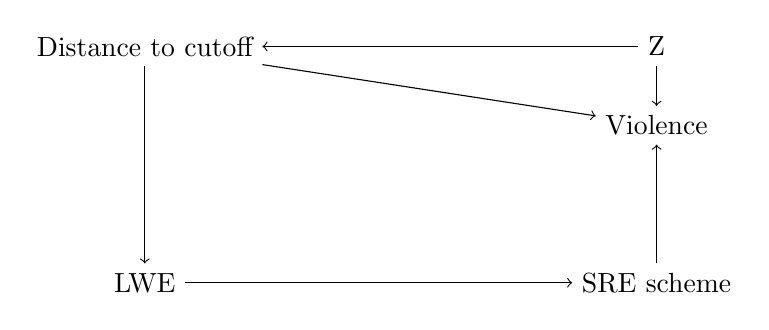
\begin{tikzpicture}
\node (v0) at (-1.5,0) {LWE};
\node (v1) at (5,0) {SRE scheme};
\node (v2) at (5,2) {Violence};
\node (v3) at (-1.5,3) {Distance to cutoff};
\node (v4) at (5,3) {Z};
\draw [->] (v1) edge (v2);
\draw [->] (v0) edge (v1);
\draw [->] (v3) edge (v0);
\draw [->] (v3) edge (v2);
\draw [->] (v4) edge (v3);
\draw [->] (v4) edge (v2);
\end{tikzpicture}
\end{adjustbox}
\end{figure*}
\column{0.5\textwidth}
\begin{figure}
\includegraphics[height= 0.5\textheight, center]{theeffect2.png}
\caption*{\tiny{Source: The Effect, Nick Huntington-Klein}}
\end{figure}
\end{columns}
\end{frame}

\begin{frame}{Model}
\only<1->{\begin{block}{Linear}
$riotspost18_{i} = \beta_{0} + \beta_{1}L_{i} + \beta_{2}D_{i} + \beta_{3}L_{i}D_{i} + \mu_{i}$
\end{block}}
\only<2->{$\beta_{1}$ is the coefficient of interest.}
\only<3->{\begin{block}{2nd order polynomial}
$riotspost18_{i} = \beta_{0} + \beta_{1}L_{i} + \beta_{2}D_{i} + \beta_{3}{D_{i}}^2 + \beta_{4}L_{i}D_{i} + \beta_{5}L_{i}(D_{i})^2 + \mu_{i}$
\end{block}}
\only<4->{Following the recommendations of [Gelman and Imbens, 2019], I do not check for higher order polynomials greater than two.}
\end{frame}

\begin{frame}{rdrobust}
\begin{itemize}
\item Bias correction
\item MSE optimised bandwidth selection
\item Triangularly weighted kernel
\item Heteroskedasticity robust standard errors
\item Controls
\item Restricting geographical area under study
\end{itemize}
\begin{block}{Estimating model with controls}
$riotspost18_{is} = \beta_{0} + \beta_{1}L_{i} + \beta_{2}D_{i} + \beta_{3}L_{i}D_{i} + X_{i}\gamma + \lambda_{s} + \mu_{i}$
\end{block}
\end{frame}

\section{Results}

\begin{frame}{Main RD estimates}
 \begin{columns}
\column{0.65\textwidth}
  \begin{table}
  \caption{State-wise Bias-corrected Robust RD Estimates} 
 \label{main} 
\begin{adjustbox}{width= 0.95\textwidth}
\begin{tabular}{@{\extracolsep{5pt}} lcccccccc} 
\\[-3.5ex]\hline 
\hline \\[-1.8ex] 
 & Estimate & $95\%$ CI & Std. Error & Robust P-Value & Obs & Eff. Obs & Bandwidth & Covs \\ 
\hline \\[-1.8ex] 
ANDHRA PRADESH & $0.217$ & $[-0.415,0.849]$ & $0.322$ & $0.500$ & $635$ & $324$ & $53.525$ & Yes\\ 
ANDHRA PRADESH & $0.172$ & $[-0.672,1.016]$ & $0.431$ & $0.689$ & $635$ & $276$ & $34.799$ & No\\ 
\hline \\[-1.8ex] 
BIHAR & $4.729$ & $[-44.435,53.893]$ & $25.084$ & $0.850$ & $79$ & $27$ & $13.610$ & Yes\\ 
BIHAR & $9.501$ & $[-13.902,32.904]$ & $11.940$ & $0.426$ & $79$ & $36$ & $19.468$ & No\\ 
\hline \\[-1.8ex] 
\textbf{CHHATISGARH} & $\textbf{-3.552}$ & $\textbf{[-5.282,-1.822]}$ & $\textbf{0.883}$ & $\textbf{0.0001}$ & $\textbf{117}$ & $\textbf{30}$ & $\textbf{14.651}$ & \textbf{Yes}\\ 
CHHATISGARH & $-1.412$ & $[-3.512,0.687]$ & $1.071$ & $0.187$ & $117$ & $32$ & $16.075$ & No\\ 
\hline \\[-1.8ex] 
\textbf{JHARKHAND} & $\textbf{0.941}$ & $\textbf{[-0.503,2.385]}$ & $\textbf{0.737}$ & $\textbf{0.201}$ & $\textbf{256}$ & $\textbf{58}$ & $\textbf{11.552}$ & \textbf{Yes}\\ 
JHARKHAND & $0.750$ & $[-0.626,2.126]$ & $0.702$ & $0.285$ & $256$ & $68$ & $14.457$ & No\\ 
\hline \\[-1.8ex] 
KERALA & $2.700$ & $[-45.900,51.300]$ & $24.796$ & $0.913$ & $61$ & $13$ & $12.488$ & Yes\\ 
KERALA & $14.533$ & $[-40.786,69.851]$ & $28.224$ & $0.607$ & $61$ & $11$ & $11.379$ & No\\ 
\hline \\[-1.8ex] 
MADHYA PRADESH & $-2.205$ & $[-6.349,1.939]$ & $2.115$ & $0.297$ & $259$ & $24$ & $36.846$ & Yes\\ 
MADHYA PRADESH & $-3.026$ & $[-11.596,5.545]$ & $4.373$ & $0.489$ & $259$ & $22$ & $32.865$ & No\\
\hline \\[-1.8ex] 
MAHARASHTRA & $-1.031$ & $[-2.272,0.209]$ & $0.633$ & $0.103$ & $329$ & $33$ & $29.596$ & Yes\\ 
MAHARASHTRA & $-1.643$ & $[-3.477,0.191]$ & $0.936$ & $0.079$ & $329$ & $29$ & $25.233$ & No\\ 
\hline \\[-1.8ex] 
\textbf{ODISHA} & $\textbf{-6.024}$ & $\textbf{[-10.725,-1.323]}$ & $\textbf{2.398}$ & $\textbf{0.012}$ & $\textbf{89}$ & $\textbf{36}$ & $\textbf{22.268}$ & \textbf{Yes}\\ 
ODISHA & $-3.066$ & $[-7.914,1.783]$ & $2.474$ & $0.215$ & $89$ & $36$ & $23.332$ & No\\ 
\hline \\[-1.8ex] 
TELANGANA & $-0.024$ & $[-0.845,0.797]$ & $0.419$ & $0.954$ & $429$ & $160$ & $25.251$ & Yes\\ 
TELANGANA & $-0.086$ & $[-1.016,0.845]$ & $0.475$ & $0.857$ & $429$ & $170$ & $27.715$ & No\\ 
\hline \\[-1.8ex] 
UTTARPRADESH & $-5.811$ & $[-12.568,0.946]$ & $3.448$ & $0.092$ & $245$ & $54$ & $65.202$ & Yes\\ 
UTTARPRADESH & $-6.571$ & $[-18.715,5.574]$ & $6.196$ & $0.289$ & $245$ & $52$ & $60.551$ & No\\ 
\hline \\[-1.8ex] 
\end{tabular} 
\end{adjustbox}
\end{table}
\column{0.35\textwidth} 
\begin{itemize}
\item Catch-up effect
\item Rollout and/or focused treatment
\item Violence as a proxy
\end{itemize}
\end{columns}
\end{frame}

\begin{frame}{Aggregated RD estimate}
\begin{table}[!htbp] \centering 
  \caption{Aggregated Bias-corrected Robust RD Estimates} 
\label{total}
\begin{adjustbox}{width=0.75\textwidth}
\begin{tabular}{@{\extracolsep{5pt}} lcccccccc} 
\\[-3.5ex]\hline 
\hline \\[-1.8ex] 
 & Estimate & $95\%$ CI & Std. Error & Robust P-Value & Obs & Eff. Obs & Bandwidth & Covs \\ 
\hline \\[-1.8ex] 
LWE STATES & $-0.471$ & $[-1.187,0.245]$ & $0.365$ & $0.197$ & $2527$ & $1194$ & $63.942$ & Yes\\ 
LWE STATES & $-0.209$ & $[-1.364,0.947]$ & $0.590$ & $0.724$ & $2527$ & $1154$ & $59.723$ & No\\ 
\hline \\[-1.8ex] 
\end{tabular} 
\end{adjustbox}
\caption*{\textit{Notes}. Standard errors are clustered by state.}
\end{table}
\end{frame}

\begin{frame}{Placebo test}
\begin{table}[!htbp] \centering 
  \caption{Placebo Test} 
  \caption*{Outcome variable: Total riots before 2018 (2016 to 2017)}
\label{placebo}
\begin{adjustbox}{width=0.75\textwidth}
\begin{tabular}{@{\extracolsep{5pt}} lcccccccc} 
\\[-3.5ex]\hline 
\hline \\[-1.8ex] 
 & Estimate & $95\%$ CI & Std. Error & Robust P-Value & Obs & Eff. Obs & Bandwidth & Covs \\ 
\hline \\[-1.8ex] 
CHHATISGARH & $-0.068$ & $[-1.159,0.023]$ & $0.046$ & $0.142$ & $117$ & $32$ & $16.280$ & Yes\\ 
ODISHA & $-0.326$ & $[-1.602,0.949]$ & $0.651$ & $0.616$ & $89$ & $40$ & $26.840$ & Yes\\ 
\hline \\[-1.8ex] 
\end{tabular} 
\end{adjustbox}
\caption*{\textit{Notes}. Standard errors are heteroskedasticity robust.}
\end{table}
\end{frame}

\section{Conclusion}

\begin{frame}{Conclusion}
\begin{itemize}
\item I find that violence post 2018 is lower by approximately 4 events in Chhattisgarh and 6 events in Odisha for the treated subdistricts
\item Intriguing case of Jharkhand
\item Shortcomings: Filtering for LWE, Non-euclidean distance, Two-running variable approach
\item Way forward: Village/Town level, Alternate sources of Violence
\end{itemize}
\end{frame}

\section{}
\begin{frame}[plain]
\frametitle{Fin.}
  \centering \Huge
  \textbf{Thank You}
\end{frame}
\end{document} 
